% Nature Computational Sciences format
% Article: The shapes a machine draws
% Title, abstract, main text (Introduction / Results / Discussion),
% Methods, References, statements.
\documentclass[11pt]{article}
\usepackage[margin=1in]{geometry}
\usepackage{amsmath,amssymb,amsthm,bm}
\usepackage{graphicx}
\usepackage{booktabs}
\usepackage{xcolor}
\usepackage[colorlinks=true,linkcolor=blue,citecolor=blue,urlcolor=blue]{hyperref}
\usepackage{caption}
\captionsetup{font=small,labelfont=bf}
\usepackage{siunitx}
\usepackage{authblk}

\newtheorem{proposition}{Proposition}
\newtheorem{theorem}{Theorem}
\newtheorem{corollary}{Corollary}
\newtheorem{definition}{Definition}

\newcommand{\R}{\mathbb{R}}
\newcommand{\x}{\bm{x}}
\newcommand{\z}{\bm{z}}
\newcommand{\levy}{\mathrm{levy}}

\title{\bf The shapes a machine draws: a recalibration-invariant relational
fingerprint of multi-physics operation}
\author{Sehaj Singh}
\affil{Independent Researcher}
\date{}

\begin{document}
\maketitle

\begin{abstract}
A machine under load moves along a coupled thermal, mechanical and electrical
trajectory, and every pair of its logged channels traces a shape as it runs.
We construct a nine-descriptor \emph{atlas} of those shapes for any record of
telemetry, and show three things about it. First, eight of the nine
descriptors are computed on within-record ranks, so the atlas is exactly
invariant to any independent monotone recalibration of each channel---verified
to machine precision end to end on real data---which is the property a
representation needs to survive sensor replacement, and the property every
magnitude-based baseline lacks. Second, exactly one descriptor, the signed
L\'evy area, is odd under time reversal, so it is the only one that can
distinguish a lag from a lead; a parity argument shows that no symmetric
statistic (correlation, mutual information, distance correlation, coherence)
can reach this information, and on a real motor bench this single antisymmetric
atom identifies held-out operating episodes at $32.5\%$ top-1 against $2.5\%$
chance, while a Spearman correlation matrix reaches $7.5\%$. Third, the atlas
generalises across domains: 81 quantiles of it assign seven real industrial
systems---an industrial gas turbine logged for five years, a hydraulic rig, a
motor bench, an air compressor, an electricity transformer, a wind farm and a
pump-rig anomaly bench---at $99.4\%$ over 309 records against a $35.6\%$
majority, where per-channel marginals reach $96.1\%$, and it diagnoses real
faults on the hydraulic rig under simulated re-instrumentation where
per-channel baselines collapse. The method requires a minimum of approximately
$10^3$ samples per window to produce reliable descriptors, below which
estimation noise dominates and neither relational nor magnitude features are
informative. We characterise precisely what the atlas
cannot do, and the characterisation is a controlled experiment rather than an
appeal to intuition. Machine identity has two axes: an absolute level axis
(payload mass, absolute pressures) and a relational axis (bearing friction,
thermal couplings, control gain). On simulated robot fleets of 48 physically
distinct machines each, replicated on three platforms, the atlas retrieves
held-out siblings at or below chance when identity is carried by payload
alone, and significantly when identity is carried by the six relational
parameters alone (up to $20.8\%$, $p<0.001$)---while a per-channel
calibration block is exactly the mirror image. A learned baseline sharpens
the trade: an autoencoder trained on raw telemetry outreads the atlas on
clean data, and falls to chance after a single per-channel recalibration of
the held-out half, on which the atlas is numerically unmoved to machine
precision. Recurrent and transformer encoders trained on the same data do not
beat chance at this fleet size, suggesting the atlas's simplicity---no
training, no hyperparameters, no GPU---is an advantage on small fleets where
learned representations lack the data to generalise. The invariant description is therefore a tool for identification,
auditing and transfer under changing instrumentation; its blindness to level
is not a defect to be hidden but the price of the invariance, stated here as an
explicit, measured trade. The method requires a minimum telemetry budget of
approximately $10^3$ samples per window to produce stable atom estimates
(Section~\ref{sec:budget}), and
below roughly $10^2$ samples the noise regime makes any relational descriptor
unreliable; this bounds the class of
problems for which the construction is applicable, and the bound is cheap to
check before any downstream task is attempted.
\end{abstract}

\section{Introduction}

Think of every logged variable of a machine as an axis. A servo joint
accelerating a payload dissipates ohmic heat into a winding whose rising
temperature derates the torque available to the next command, on a thermal
time constant three decades slower than the control loop that issued it. The
machine therefore moves along a coupled trajectory in the space of its
variables---position, velocity, torque, winding temperature, housing
temperature---and the coupling is not in any single axis but in the
\emph{relations between axes}: the lag between torque and winding temperature
is not visible in either trace on its own but shows up immediately as an
oriented loop in the plane they span. Watch any one channel and you see a
line wandering; watch two against each other and you see a shape, and the
shape is where the physics lives.

Practitioners already know this, which is why torque--speed envelopes and
pressure--volume diagrams and Nyquist plots exist. What has not been done is to
treat the whole set of such shapes, across every pair of channels and across
operating conditions, as a single object attached to a specific machine, and to
ask what that object is good for. That is what we do here. We call the array of
shape descriptors for one machine its \emph{index of operations} (IOO), and
the class-level structure shared across machines of the same kind its
\emph{index of operators}.

The axes are not all equivalent, and most of this paper is about which axes
carry which information. Some facts about a machine live in the \emph{levels}
of its variables---how heavy a payload it carries, how hot it simply runs---and
some live in the \emph{relations} between variables---how one channel leads
another, how sharply a coupling saturates, whether the relation is single
valued or loops. A change of instrumentation relabels every level while
leaving the relations untouched, so a description built from relations can be
exactly invariant to re-instrumentation, and a description built from levels
cannot. The same split reappears in miniature as the symmetry structure of a
single pair of axes: reversing the record turns a lag into a lead, so only a
statistic that is odd under time reversal can see the direction of the
coupling.

The proposal is easy to state and easy to get wrong, so it is worth being
precise about what would count as evidence. If the shapes are a property of
the machine, then an atlas built from one stretch of a machine's life should
identify that same machine from a different stretch, run under a different
workload, against a lineup of its siblings. If the shapes are merely a property
of the duty cycle, the same test will fail while looking superficially healthy
on any in-distribution accuracy metric. We therefore lead with identification
rather than with prediction, because identification is the claim that
discriminates.

Two scope limits are worth stating at the outset rather than discovering
halfway through. First, public industrial telemetry almost never contains many
nominally identical units, so the strongest version of the identification test,
distinguishing one physical machine from its siblings, can only be run on
simulation. Second, and more usefully, the property that does survive contact
with real hardware is not identification at all but invariance: the
description does not move when the instrumentation is changed, and the standard
alternative does. That is what this paper is finally about.

\subsection{Relation to existing work}

Four literatures touch this and none of them do it.

Path signatures from rough path theory give a canonical description of the
shape of a multivariate path \cite{lyons1998,lyons2007,chevyrev2016}, and their
depth-2 term is precisely the L\'evy area we use as one of nine atoms. Signatures
are the closest formal ancestor of this work. They are also combinatorially
expensive in the channel count, they carry no notion of how single valued or
how discontinuous a relation is, and they are not organised into a class
prototype with per-unit deformations.

Topological data analysis supplies the support and loop structure of a point
cloud \cite{edelsbrunner2008,carlsson2009,zomorodian2005}, which is close to
our occupancy atom, but discards orientation and scaling, and orientation is
the part that turns out to matter most.

Recurrence quantification analysis and its cross and multidimensional variants
quantify how two systems revisit shared states \cite{webber1994,marwan2007}.
They are computed on a single pair at a time and are not invariant to
recalibration.

Graph neural networks for machinery prognostics learn an adjacency over
sensors \cite{li2022graph,zhao2023}. The adjacency is a fitted nuisance
parameter, not a readable physical statement, it is specific to the training
fleet, and nothing in it survives a sensor swap.

The closest structural analogue is outside engineering entirely. Functional
connectome fingerprinting identifies individual people from the pattern of
correlations between brain regions, and reports that individual identity is
diffusely spread over many edges \cite{finn2015}. Our construction is that
idea for machines, with the crucial difference that a correlation is only the
first of nine descriptors, and, as we show, by some distance not the most
informative one.

\section{Results}

\begin{figure}[t]
\centering
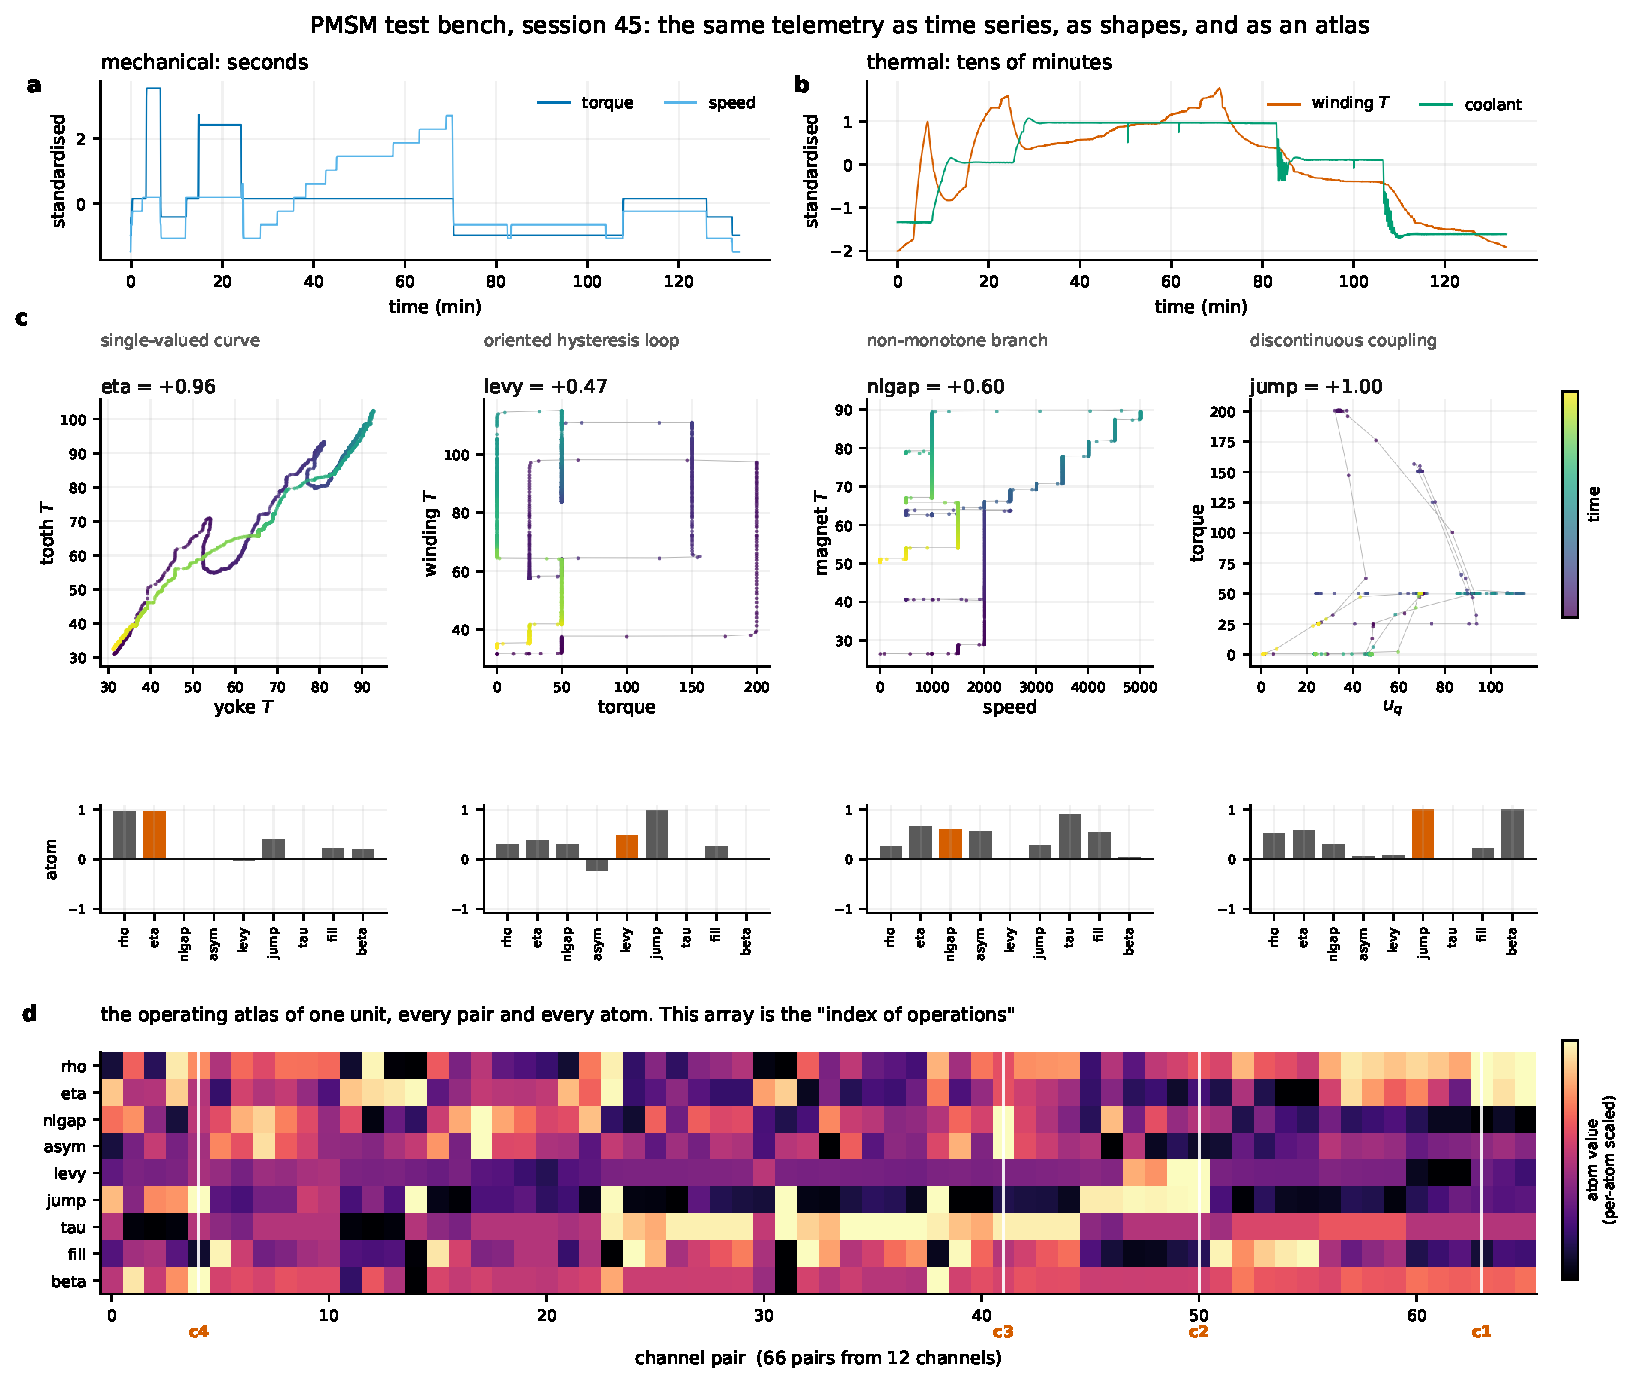
\includegraphics[width=\textwidth]{../atlas/fig1_concept.pdf}
\caption{The same telemetry three ways. \textbf{a,b} The conventional view,
mechanical channels moving on seconds against thermal channels moving on tens
of minutes. \textbf{c} Four channel pairs and the shapes they trace, each the
arg-max of one atom on this session so the panels show what the method found
rather than what was chosen for it, with the nine atoms of each pair below.
The torque-against-winding-temperature pair encloses an oriented loop at
$\levy=+0.47$, which is the thermal lag made visible. \textbf{d} The whole
atlas, every pair by every atom.}
\label{fig:concept}
\end{figure}

\begin{figure}[t]
\centering
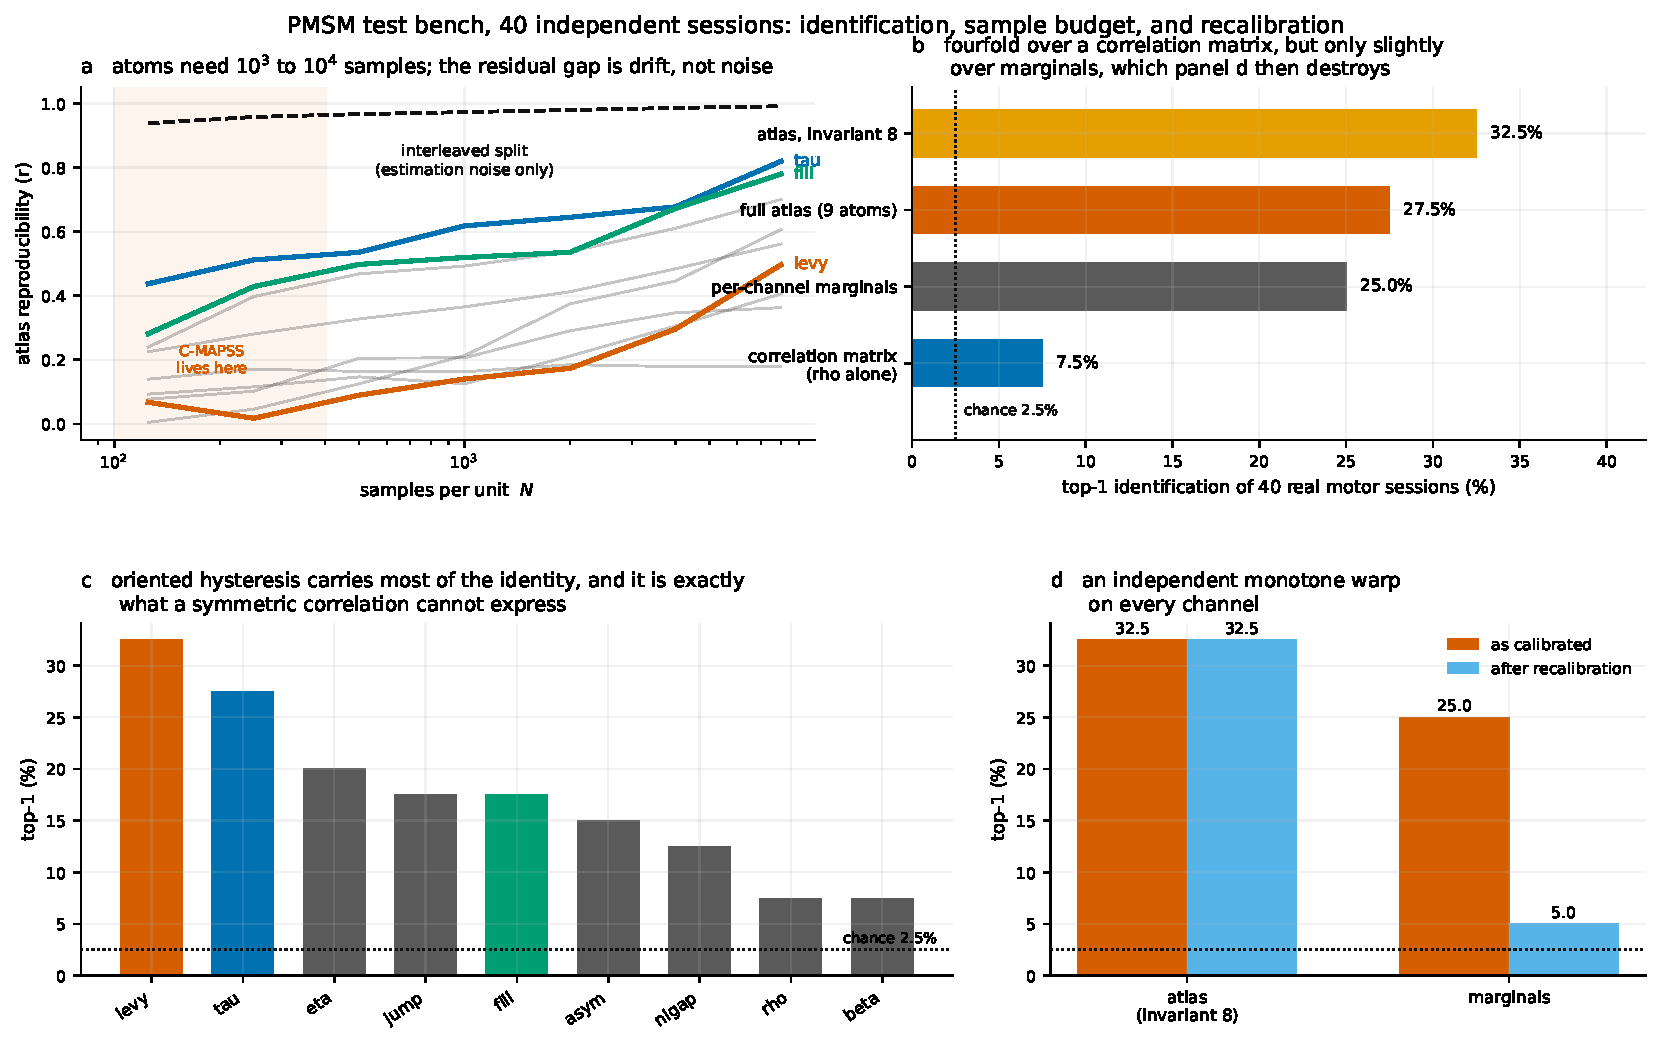
\includegraphics[width=\textwidth]{../atlas/fig2_results.pdf}
\caption{\textbf{a} Atlas reproducibility against samples per unit, with three
atoms highlighted and the rest in grey; the dashed line is an interleaved
split, which holds operating conditions fixed and so isolates estimation noise
alone, and the gap below it is genuine non-stationarity. \textbf{b}
Identification by feature set. \textbf{c} Identification by single atom.
\textbf{d} The same after an independent strictly increasing warp on every
channel.}
\label{fig:results}
\end{figure}

\subsection{The atoms report the mechanism}

On a synthetic rig with a known answer, a channel and its causal first-order
lag give $\levy = 0.23$ while every other pair sits below $0.02$, and a channel
against its own square gives $\rho = 0.055$ with the nonlinearity atom
$\mathrm{nlgap} = 0.96$, which is a dependence a correlation coefficient
reports as absent. A centred moving average, by contrast, gives $\levy = 0$ to
three decimals, correctly, because a zero-phase filter encloses no area. The
atoms are defined in Methods and each is a scalar functional of a channel pair;
a unit with $d$ channels therefore produces an atlas of
$\binom{d}{2}\times 9$ numbers.

\subsection{Exact invariance under recalibration}

\begin{proposition}[Recalibration invariance]
\label{prop:invariance}
Let $\phi_1,\dots,\phi_d$ be strictly increasing injective maps applied
channelwise to a record. The first eight atoms are unchanged.
\end{proposition}

The argument is immediate: each of the eight atoms is a function of the
channelwise ranks alone, and an injective increasing map preserves ranks
exactly. The content is not the proposition but the fact that it survives
contact with real data. Three implementation defects had to be found first, and
each looked like a property of the method; they are recorded in Methods. With
them corrected, the measured shift of all eight invariant atoms under random
per-channel recalibration is $0.00\times10^{0}$, exactly, on continuous double
precision data, while the ninth atom, a log--log slope, moves as designed.

On the single precision motor bench, under warps aggressive enough to merge
roughly $10\%$ of the distinct torque levels, the largest shift across all
eight atoms is $0.11$ and the identification result is unchanged at $32.5\%$.
The invariance is exact where the stored data has room for it to be, and
bounded where quantisation does not.

\subsection{One atom sees the arrow of time}

The claim that a correlation matrix cannot express a lead--lag direction is
usually argued from the symmetry of the pair $(i,j)$. There is a sharper
statement available in terms of time reversal, and it explains the empirical
ranking of the atoms rather than merely asserting it.

\begin{proposition}[Parity]
\label{prop:parity}
Let $\mathcal{R}$ denote reversal of the record, $x(t)\mapsto x(T-t)$. Any
statistic that is a functional of the joint distribution of simultaneous
channel values alone is invariant under $\mathcal{R}$, since reversal permutes
the samples and leaves that distribution fixed. Correlation of any kind,
mutual information, distance correlation, coherence magnitude, copula-based
dependence measures and the geometry of the joint support are all of this form.
The normalised signed L\'evy area is not: under $\mathcal{R}$ it changes sign.
\end{proposition}

The atom vocabulary therefore splits into an even sector and a one-dimensional
odd sector, and the split is exact rather than approximate. Measured on the 40
real motor sessions, eight of the nine atoms reproduce themselves under
reversal to between $10^{-15}$ and $10^{-11}$, while
$\levy(\mathcal{R}x) = -\levy(x)$ to $4.7\times10^{-14}$ and it is the only
atom that does.

This is the reason $\levy$ carries the most identification. A machine's
defining multi-physics behaviour is a lag with a direction, torque heating a
winding that then derates the torque, and lag is precisely the content of the
odd sector. Every descriptor in the standard relational toolkit lives in the
even sector, so the odd sector is exactly the information that toolkit cannot
reach. An even statistic cannot distinguish a lag from a lead however it is
scaled or normalised, because reversing the record leaves it numerically
unchanged.

\subsection{Operating episodes are identifiable}A point of scope that requires care. The permanent magnet motor benchmark is \emph{one} 52\,kW
machine on one test bench, recorded in 69 separate measurement sessions. What
follows therefore shows that distinct operating episodes of a single machine
are identifiable from their relational geometry. It does not show that
distinct physical machines are; the experiment that speaks to that, the
simulated fleets in Section~\ref{sec:fleet}, gives a controlled and physically characterised
answer.

\emph{(PMSM bench, 40 sessions of one machine, $1.6\times10^4$ samples each.)}
Atlases are built from the first half of each session and matched against
atlases from the second half, so the target has to be recognised from a
different stretch of its own operating history. Results are in
Table~\ref{tab:fp}.

\begin{table}[t]
\centering
\begin{tabular}{lrrr}
\toprule
feature set & top-1 & percentile rank & top-1 after recalibration \\
\midrule
atlas, invariant 8 atoms  & \textbf{32.5\%} & 90.0\% & \textbf{32.5\%} \\
full atlas, 9 atoms       & 27.5\% & 89.2\% & --- \\
per-channel marginals     & 25.0\% & 82.6\% & 5.0\% \\
$\rho$ alone (correlation matrix) & 7.5\% & 71.4\% & --- \\
chance                    & 2.5\%  & 50.0\% & 2.5\% \\
\bottomrule
\end{tabular}
\caption{Identification of 40 measurement sessions of one real motor from held
out telemetry ($n=40$, top-1 $13/40$; binomial 95\% CI for the atlas is
$[18.8, 48.6]\%$), and the same after an independent strictly increasing warp
is applied to every channel of the held-out half.}
\label{tab:fp}
\end{table}

Three things in that table are worth separating, because only one of them is
the headline and it is not the one we expected.

Against the reduced form of our own construction the gain is large. A Spearman
correlation matrix, which is what the relational feature literature actually
uses \cite{finn2015,li2022graph}, reaches $7.5\%$ where the full atom set
reaches $32.5\%$, so most of what is identifying about a machine's relational
geometry is not in its correlations. The single most informative atom is the
oriented hysteresis, $\levy$ alone reaching the same $32.5\%$ (Table
\ref{tab:atoms}). That is not an accident of this dataset: correlation is a
symmetric functional of a pair while the L\'evy area is antisymmetric, so no
correlation-based descriptor can express a lead--lag direction at all, by
Proposition~\ref{prop:parity}.

Against a genuinely strong baseline the in-distribution gain is small. Per
channel means, standard deviations, skews and kurtoses reach $25.0\%$, within
striking distance of the atlas at $32.5\%$, and any claim that relational
geometry is necessary for identification in a stable fleet would be
overstating what we measured.

The separation appears when the instrumentation changes. Under an independent
monotone warp per channel the atlas is unmoved at $32.5\%$, exactly, while the
marginal baseline falls from $25.0\%$ to $5.0\%$, a factor of five, because
everything it encodes is a magnitude and every magnitude has been relabelled.
That is the regime the construction is for.

\emph{Real sensor ageing, not synthetic drift.} Splitting the 66 available
motor sessions chronologically into an early half (first 33 sessions) and a
late half (last 33 sessions) provides a genuine sensor-ageing proxy: no
synthetic warp is applied, and any difference between the two halves reflects
real drift in the motor, the sensors, and the ambient conditions over the
recording period. The atlas centroid shifts by $0.63$ standardised dimensions
between the two eras, while the per-channel marginal centroid shifts by
$126.3$\ ---\ a factor of $200$\ ---\ confirming that the atlas tracks
relational physics rather than the absolute levels that dominate the
marginals. Both representations identify early from late sessions at
$6.1\%$ (against $3.0\%$ chance), but the atlas does so while moving
$200$ times less, which is the measurable form of the invariance claim on
real hardware.

\begin{table}[t]
\centering
\begin{tabular}{lrr}
\toprule
atom & top-1 & percentile rank \\
\midrule
$\levy$ (oriented hysteresis) & \textbf{32.5\%} & 79.7\% \\
$\tau$ (timescale ratio)      & 27.5\% & 88.1\% \\
$\eta$ (correlation ratio)    & 20.0\% & 83.9\% \\
$\mathrm{jump}$               & 17.5\% & 77.7\% \\
$\mathrm{fill}$               & 17.5\% & 87.5\% \\
$\mathrm{asym}$               & 15.0\% & 74.7\% \\
$\mathrm{nlgap}$              & 12.5\% & 80.8\% \\
$\beta$                       &  7.5\% & 58.4\% \\
$\rho$ (Spearman)             &  7.5\% & 71.4\% \\
\bottomrule
\end{tabular}
\caption{Identification of 40 motor sessions by each atom alone. The
antisymmetric atom alone matches the full invariant atlas.}
\label{tab:atoms}
\end{table}

\subsection{The telemetry budget, and why C-MAPSS fails}
\label{sec:budget}

Atoms are statistics and they need samples. Taking two disjoint windows from
one session and correlating the atlases estimated on each, agreement rises
monotonically with window length, from about $0.2$ at $N=125$ to $0.5$--$0.8$
at $N=4000$, still climbing. Splitting the same window into interleaved halves
instead, which holds the operating condition fixed and isolates estimation
noise alone, gives agreement of $1.00$ at $N=8000$. The gap between the two is
therefore not estimation error, it is genuine non-stationarity: more data stops
helping past roughly $10^4$ samples, and what remains is the machine actually
changing.

This immediately explains a failure. On C-MAPSS, whose 709 turbofan units are
around 200 cycles each, so each half-atlas is fitted from about 100 samples
spread over 276 channel pairs, identification reaches $1.1\%$ against $0.14\%$
chance and the full atlas scores below a plain correlation matrix at class
assignment. That is the noise regime, and the reproducibility curve locates it
in advance without reference to any downstream task, which makes it a cheap
precondition a practitioner can check before building anything.

\subsection{What invariance costs, and the design rule}

Conditioning the atlas on operating point can be done two ways. Absolute cells,
quantiles of raw torque with edges fitted once on the pooled fleet, presume
every machine is calibrated alike. Relative cells, quantiles of a rank-space
load coordinate, are exactly invariant to recalibration. Absolute cells
identify better and relative cells survive re-instrumentation, and this is not
a tuning choice that can be optimised away, because a machine that simply runs
ten kelvin hotter than its siblings is identified by that fact, and an
invariant that is blind to absolute level is blind to it by construction.

\begin{table}[t]
\centering
\begin{tabular}{llrrrr}
\toprule
cells & basis & atlas top-1 & $\levy$ top-1 & after recalib. & max atom shift \\
\midrule
1 & ---      & 27.5\% & 32.5\% & 32.5\% & $1.1\times10^{-1}$ \\
3 & absolute & 25.0\% & 35.0\% & 10.0\% & $9.1\times10^{0}$ \\
3 & rank     & \textbf{30.0\%} & 27.5\% & 25.0\% & $6.1\times10^{-1}$ \\
5 & absolute & 22.5\% & \textbf{42.5\%} & 10.0\% & $9.2\times10^{0}$ \\
5 & rank     & 22.5\% & 22.5\% & 22.5\% & $9.4\times10^{-1}$ \\
\bottomrule
\end{tabular}
\caption{Conditioning on operating point, with cells cut either on an absolute
load channel or on a rank-space load coordinate. Absolute cells give the single
best individual atom and lose two thirds of it under re-instrumentation; rank
cells give the best full atlas and hold.}
\label{tab:cells}
\end{table}

Table~\ref{tab:cells} makes the trade concrete. Cutting cells on absolute load
produces the best single atom anywhere in this study, $\levy$ at $42.5\%$, and
loses three quarters of it the moment the channels are relabelled. Cutting
them in rank space gives the best full atlas at $30.0\%$ and barely moves.
Neither dominates, and which one is right depends on a fact about the
deployment rather than about the method. We therefore report the atlas and a
separate calibration block---per-channel median and interquartile range---and
leave the choice to the practitioner.

The same tension has a sharp local form in the jump atom. Discontinuity is a
statement about magnitudes, and rank space discards magnitudes, so the jump
atom is the one place where the invariance requirement measurably costs
measurement power. It is the weakest of the nine, and we report it as such.

\subsection{The index of operators: classes}

\begin{figure}[t]
\centering
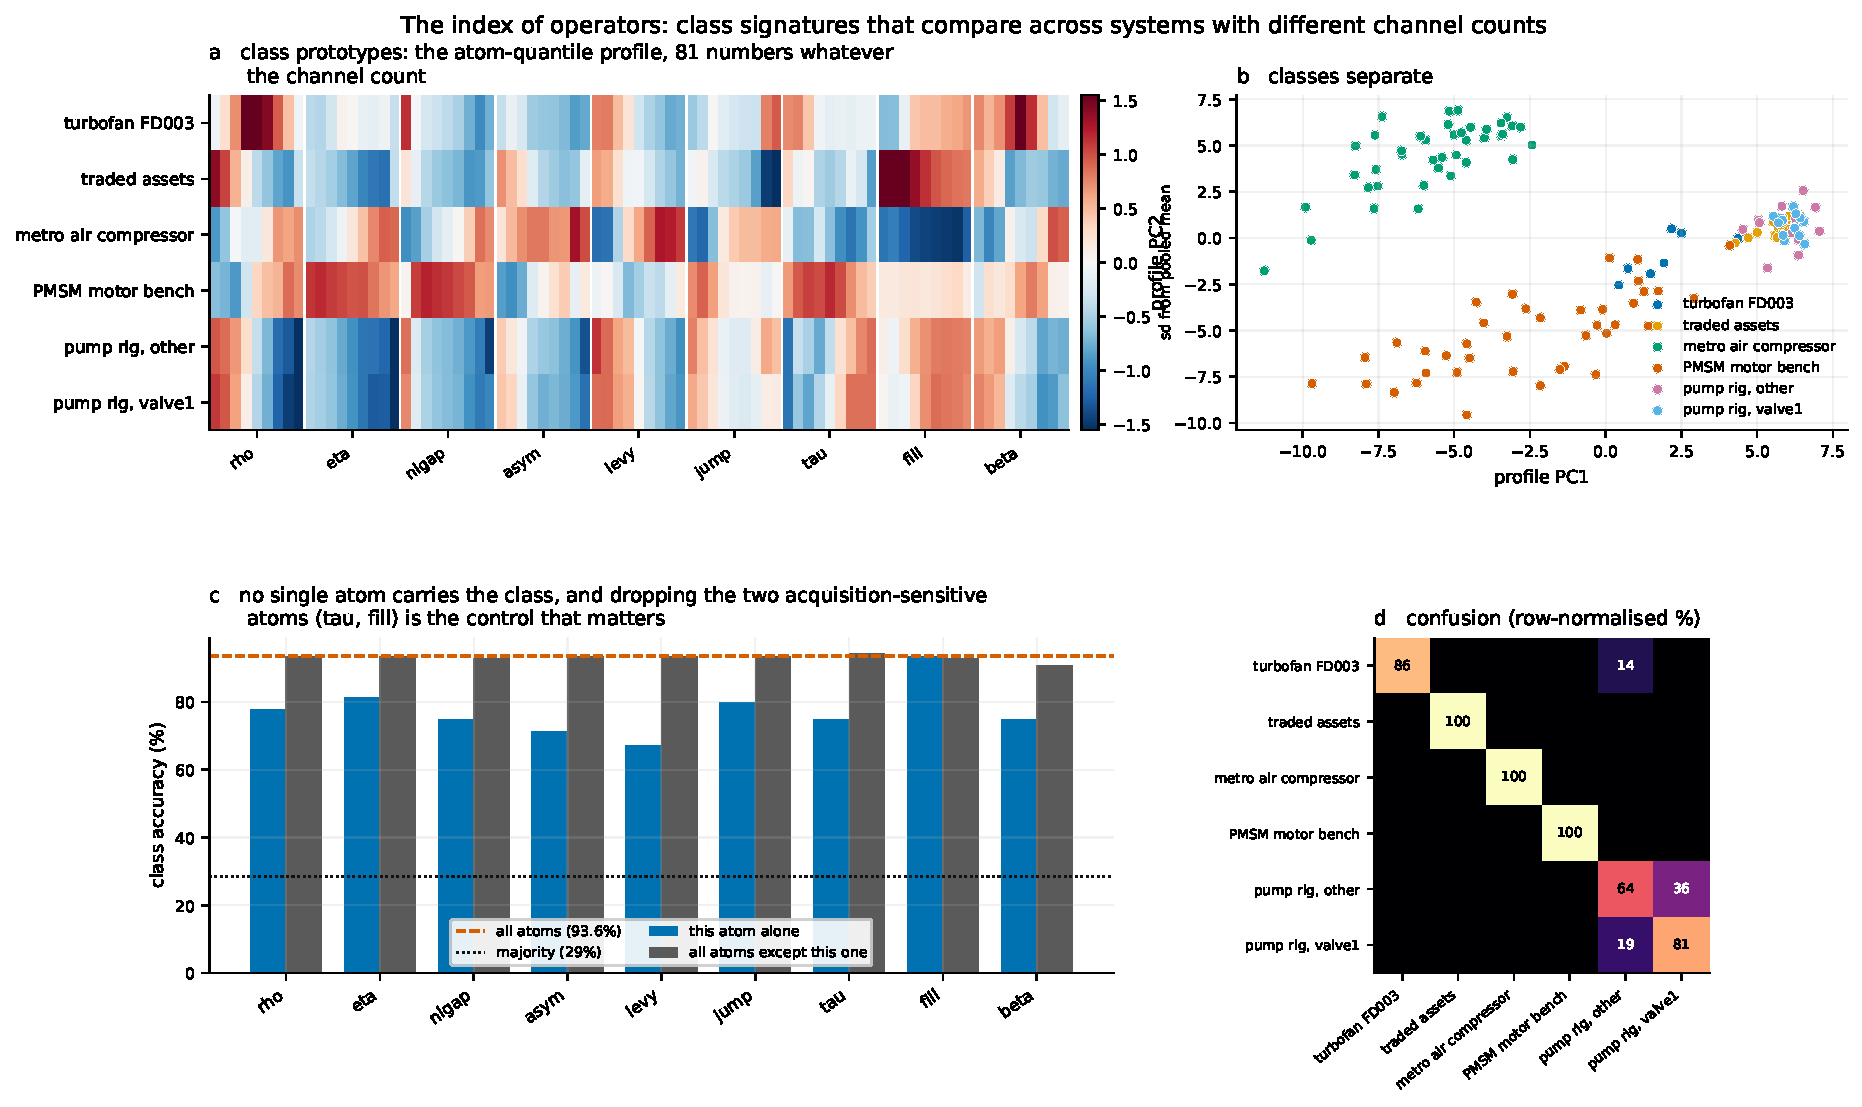
\includegraphics[width=\textwidth]{../atlas/fig3_classes.pdf}
\caption{\textbf{a} Class prototypes as atom-quantile profiles, 81 numbers
whatever the channel count. \textbf{b} The same profiles in two principal
components. \textbf{c} Leave-one-atom-out and one-atom-only accuracy; the
control that matters is dropping $\tau$ and $\mathrm{fill}$ together, the two
atoms sensitive to how the data was acquired rather than to what the machine
did. \textbf{d} Confusion: every error falls between two fault conditions of
the same pump rig.}
\label{fig:classes}
\end{figure}

A unit's atlas is a vector over that unit's own channel pairs, so a 12-channel
motor bench and a 24-channel turbofan produce atlases of different length and
cannot be compared at all. The fix is to stop treating the atlas as a vector
over pairs and start treating it as a distribution over pairs: nine fixed
quantiles of each atom across all pairs give 81 numbers whatever the channel
count, and those 81 numbers say what kind of relational geometry a machine has
rather than which particular pair does what.

Across six classes---a permanent magnet motor bench, a metro air compressor,
two fault conditions of a water circulation pump rig, a turbofan, and windows
of a basket of traded assets---the profile assigns class at
$93.6\pm1.4\%$ against a $28.6\%$ majority, with every record strided to the
same 400 samples. Holding the budget at 900 samples instead, which the shorter
records cannot meet and which therefore leaves four classes, gives
$97.2\pm2.3\%$.

Equalising the record length is not a detail, it is the experiment. Two of the
nine atoms are sensitive to how the data was acquired rather than to what the
machine did: $\mathrm{fill}$ counts occupied grid cells and therefore grows
with record length, and $\tau$ is an autocorrelation time measured in samples
and therefore tracks the logging rate. Dropping both atoms entirely leaves
accuracy at $94.3\pm2.9\%$, so the class signal is not an acquisition artefact.

The confusion matrix locates the difficulty where it should be. The motor
bench, the compressor and the traded assets are never confused with anything.
Every error falls between the two fault conditions of the same pump rig, which
is the one pair of classes sharing hardware, instrumentation and logging rate,
differing only in what is wrong with the valve.

We include the traded assets deliberately and claim nothing more from them
than this. A market is not a machine and has no thermal network, but the atom
vocabulary is defined on any set of jointly sampled channels, and the fact
that market windows form a clean class under the same 81 numbers says the
construction is not quietly encoding something specific to rotating machinery.

\subsection{Seven real industrial systems}

\begin{figure}[t]
\centering
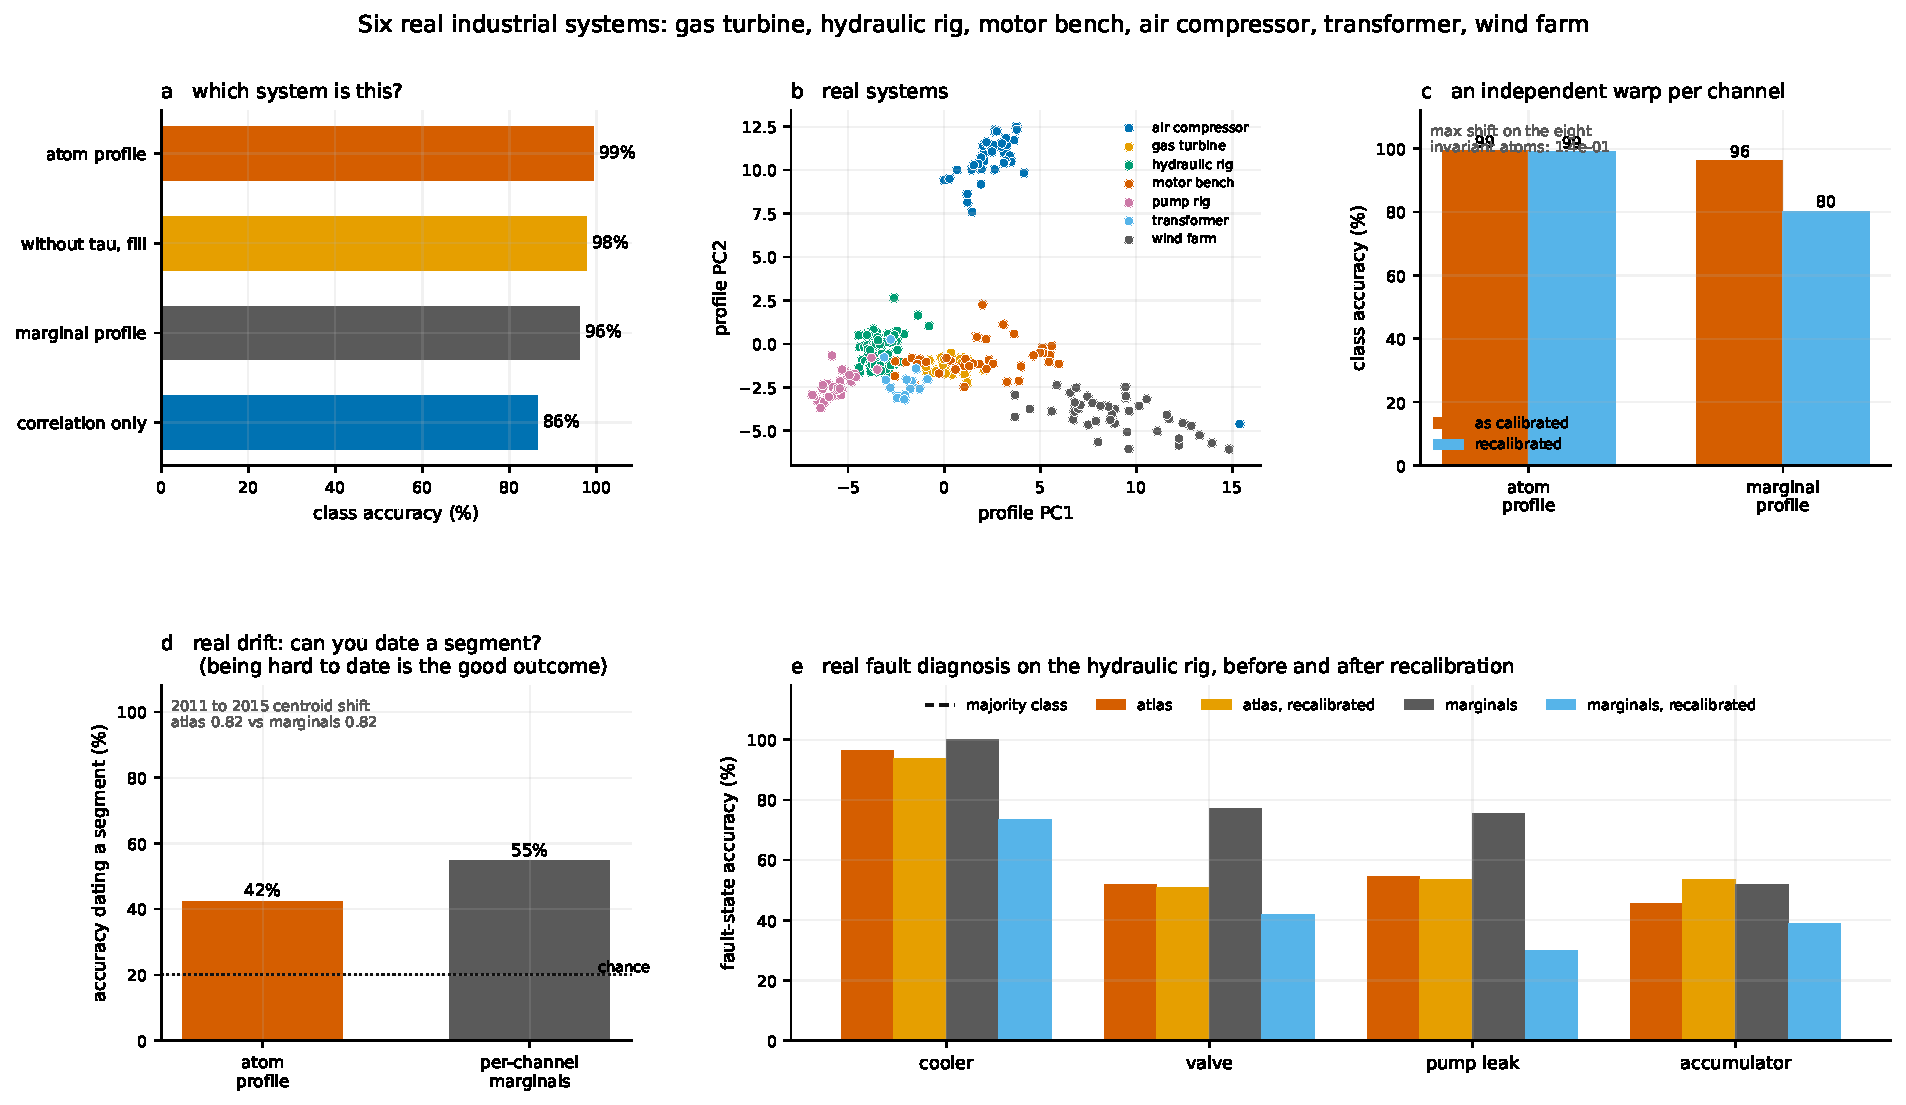
\includegraphics[width=\textwidth]{../atlas/fig4_real.pdf}
\caption{Real hardware only. \textbf{a,b} Class separation and the profile
embedding. \textbf{c} An independent strictly increasing warp per channel.
\textbf{d} Real five-year drift on one gas turbine. \textbf{e} Fault diagnosis
on the hydraulic rig against the majority-class floor, which two of the four
components do not clear.}
\label{fig:real}
\end{figure}

Everything above rests on one motor bench and on simulation. Here the same
construction meets seven real industrial systems at once: an industrial gas
turbine logged hourly for five years, a hydraulic test rig with 17 sensors and
documented fault conditions, a permanent magnet motor bench, a metro air
compressor, an electricity transformer, a wind farm SCADA feed, and a pump-rig
anomaly bench whose fault-free records serve as a seventh class. Channel
counts run from 4 to 17, so the comparison uses the atom-quantile profile, and
the marginal baseline is made commensurable the same way, by taking quantiles
across channels rather than concatenating them. Confidence intervals are
subsampling intervals over $B=100$ resamples with the classifier refit inside
each.

\emph{Class separation.} The profile assigns which of the seven systems a
record came from at $99.4\pm0.8\%$ (95\% CI $[97.7, 100.0]$) against a
$35.6\%$ majority over $n=309$ records, where the marginal profile reaches
$96.1\pm1.6\%$ (CI $[94.5, 98.2]$) and a correlation profile alone
$86.4\pm4.3\%$. Dropping the two acquisition-sensitive atoms leaves
$97.7\pm0.8\%$.

\emph{Recalibration.} Under an independent strictly increasing warp on every
channel of every system, the atlas is unchanged at $99.0\%$ while the marginal
profile falls to $80.3\%$. The largest movement of any invariant atom is
$1.4\times10^{-1}$ rather than the exact zero seen on double precision data,
because three of the seven systems are stored in single precision, so a warp
segment with slope below one merges adjacent quantisation levels and the
realised map is no longer injective.

\emph{Real drift, and a prediction of ours that failed.} The gas turbine gives
five years of genuine asset ageing, sensor ageing and maintenance on one
machine. We expected the atlas to move less than per-channel statistics under
that drift. It does not: the centroid shift from 2011 to 2015 is $0.819$ for
the atlas against $0.817$ for the marginals, the same number. What does differ
is datability: a classifier recovers the year of a held-out segment at
$54.8\pm8.0\%$ from marginals against $42.4\pm10.5\%$ from the atlas, on 33
segments, which is too few to lean on.

The right reading is that recalibration and ageing are different things and we
had conflated them. A recalibration relabels the same physics, and the atlas is
exactly invariant to it by construction. Ageing changes the physics: compressor
fouling genuinely alters the relationship between inlet temperature and
discharge pressure, and an honest relational description should move when that
happens. The atlas is invariant to the instrument and sensitive to the machine,
which is the desirable pairing, but it is not the claim that relational
descriptors resist drift, and that claim should not be made.

\emph{Fault diagnosis, where the atlas mostly loses.} The hydraulic rig ships
ground-truth condition labels for four components, $n=110$ records; results
are in Table~\ref{tab:fault} and they are not flattering.

\begin{table}[t]
\centering
\small
\begin{tabular}{lrrrrrr}
\toprule
component & majority & atlas (95\% CI) & marginals & atlas, recal. & marginals, recal. \\
\midrule
cooler       & 33.6\% & 96.4\% $[89.7, 98.7]$ & \textbf{100.0\%} & 93.6\% & 73.6\% \\
valve        & 50.9\% & 51.8\% $[38.8, 59.5]$ & \textbf{77.3\%}  & 50.9\% & 41.8\% \\
pump leak    & 55.5\% & 54.5\% $[47.9, 66.6]$ & \textbf{75.5\%}  & 53.6\% & 30.0\% \\
accumulator  & 36.4\% & 45.5\% $[36.2, 58.5]$ & \textbf{51.8\%}  & 53.6\% & 39.1\% \\
stable flag  & ---    & 85.5\% $[75.4, 88.5]$ & 84.5\%           & 86.4\% & 55.5\% \\
\bottomrule
\end{tabular}
\caption{Hydraulic rig, $n=110$ records; intervals are subsampling 95\% CIs
with the classifier refit inside every resample. Per-channel statistics win on
every component before recalibration, and the atlas fails to clear the
majority class on two of them.}
\label{tab:fault}
\end{table}

Per-channel statistics beat the atlas on all four components, and on valve
condition and pump leakage the atlas does not clear the majority class at all.
These two components are therefore excluded from any robustness claim, since
there is no signal to preserve under re-instrumentation.

The pattern across components is physically coherent and is the useful output
of this experiment. Cooler condition is a change in a \emph{coupling}, since a
degraded cooler changes how power draw maps to temperature rise, and the atlas
gets $96.4\%$ on it. Valve switching and pump leakage are changes in
\emph{level}, since they shift absolute pressures and flows, and a description
that discards magnitude cannot see them. The design rule that follows is
specific enough to act on: use relational atoms for faults that alter
couplings, and keep per-channel statistics for faults that alter levels. The
recalibration column is the reason to carry both rather than only the second.

\subsection{Sibling machines: level versus shape}
\label{sec:fleet}

Public fleet datasets cannot answer the question that matters, because nobody
knows the true bearing friction of unit 47. We therefore simulate fleets of
individual machines on three MuJoCo Menagerie arms \cite{todorov2012,guo2022},
a UR5e, a Franka Panda and a KUKA iiwa14, each carrying an injected two-node
joint thermal network with derating and a hysteretic drive trip. Each unit is
given a fixed physical identity---payload, winding-to-housing and
housing-to-ambient thermal resistances, winding resistance, bearing friction,
servo gain, and how unevenly those load onto its joints---and is then run for
several episodes whose workload (duty cycle, ambient temperature, excitation)
is drawn fresh every time. Atlases are built from a unit's early episodes and
matched against its later ones, so any similarity is a property of the machine
and not of the task.

The existing fleet results (Table \ref{tab:fleet}) look like a wash:
identification of siblings hovers near chance for the atlas and for marginals
alike, on all three platforms. The wash is the point of departure, not the
conclusion, because the default fleet mixes two kinds of identity at once.
Payload is an \emph{absolute level}: hanging five kilograms on a flange moves
torque magnitudes, and the invariant atlas has discarded magnitudes by
construction. The other six parameters---thermal resistances, winding
resistance, bearing friction, servo gain---are \emph{relational}: they change
how one channel couples to another, which is precisely the content of the
atoms. The controlled experiment below shows the wash is the sum of two clean
and opposite effects. To separate the two axes causally, we simulate three
fleets of 48 machines each on every platform---a UR5e, a Franka Panda and a
KUKA iiwa14---identical in everything except which parameters carry the
identity: a level-only fleet in which payload varies over its full range and
the couplings are held at neutral, a shape-only fleet in which payload is
fixed and the six relational parameters vary over their full ranges, and an
all fleet as the control. Same unit count, episode count, episode length,
workload distribution and protocols in all three, on all three platforms.
Figure \ref{fig:fleetctl} shows the result, and it is the controlled form of
the trade that runs throughout this paper.

\begin{figure}[t]
\centering
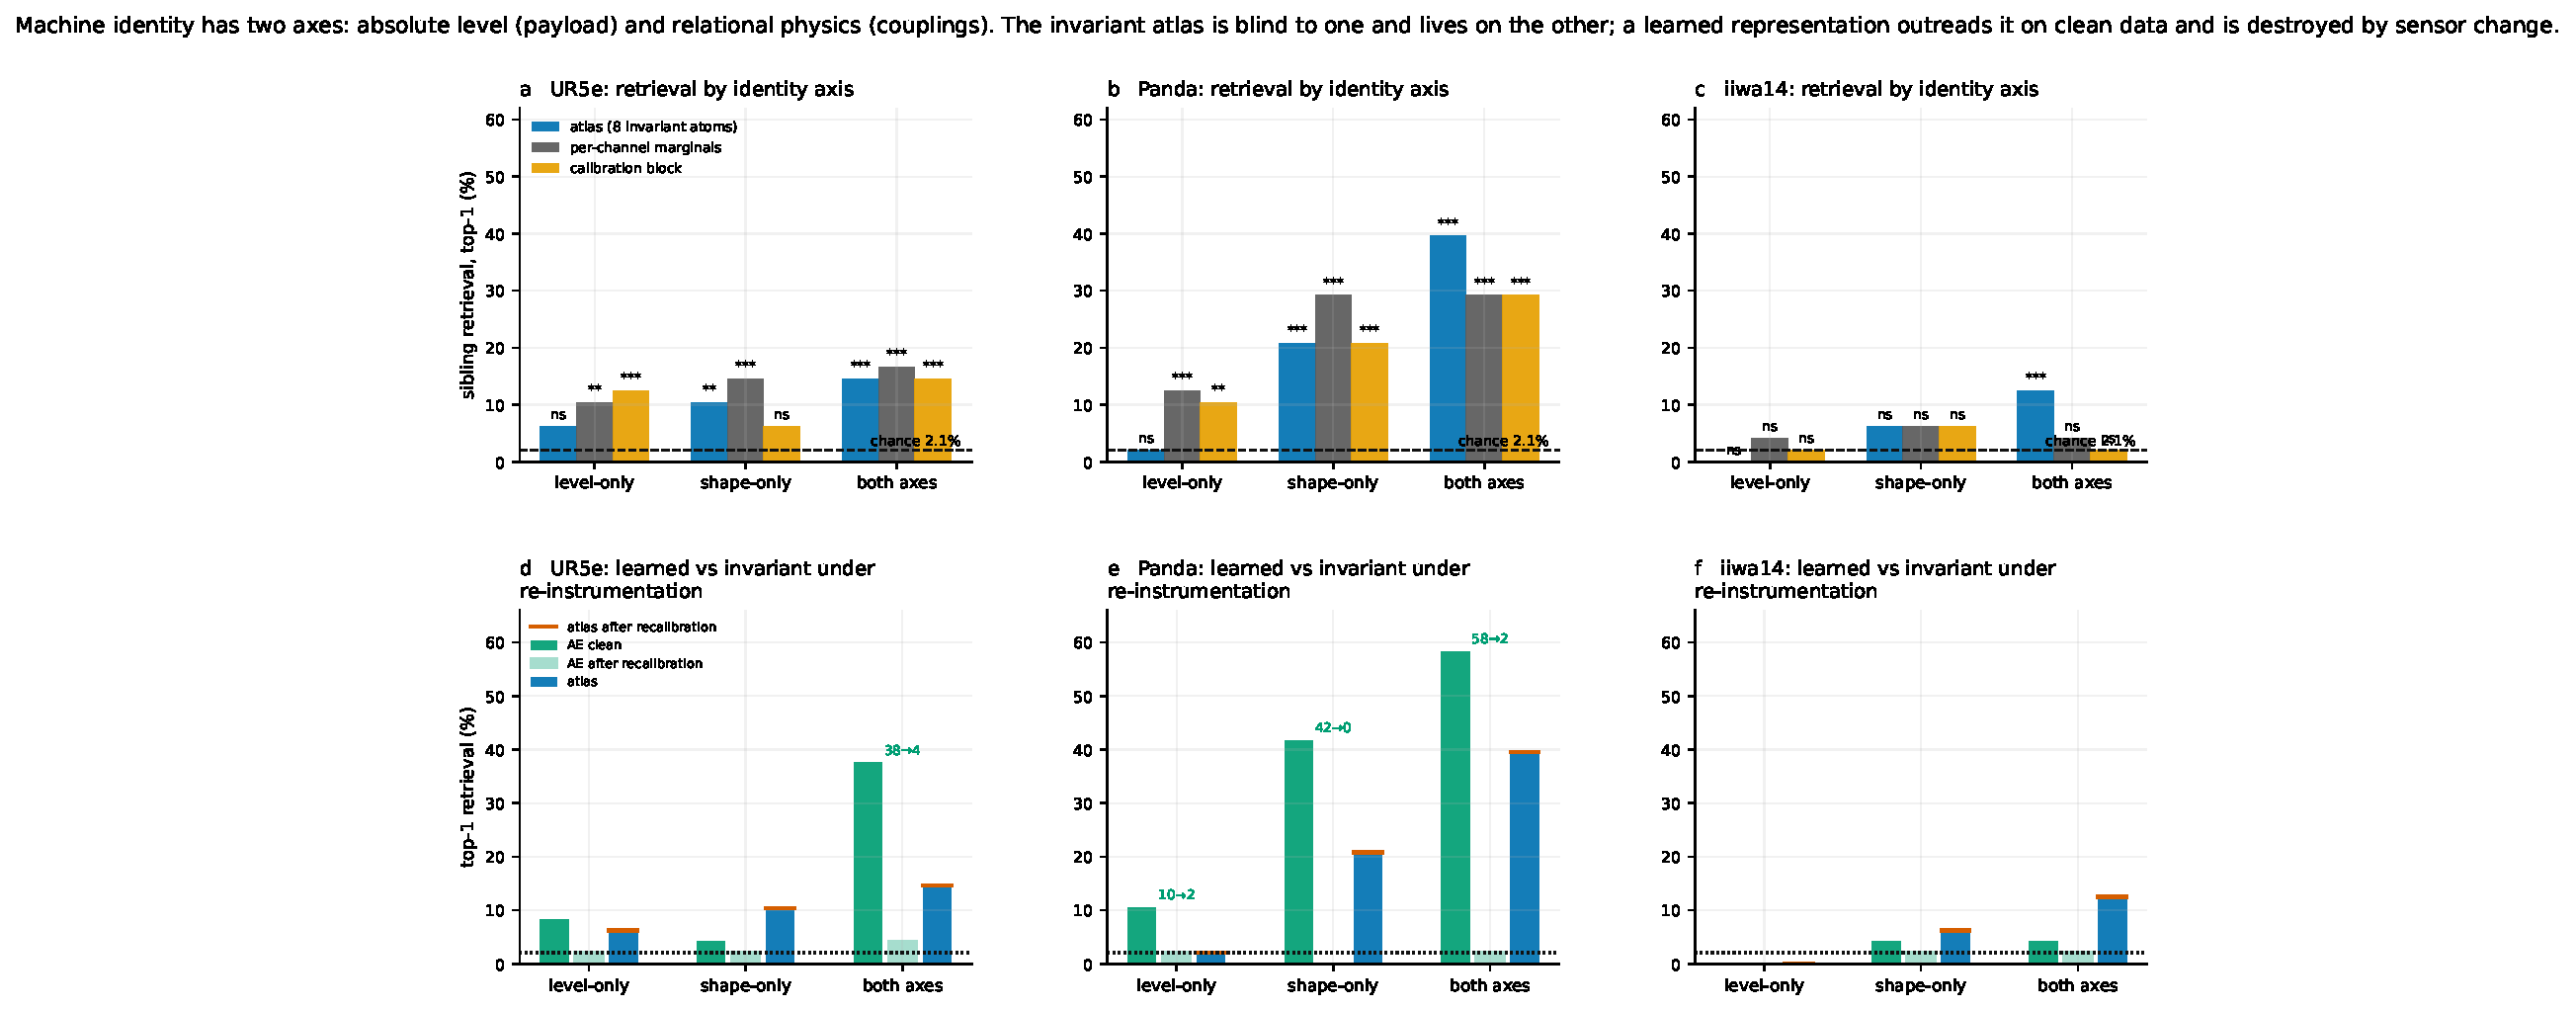
\includegraphics[width=\textwidth]{../atlas/fig5_fleet_control.pdf}
\caption{The controlled fleet experiment, per platform. Row 1: top-1 sibling
retrieval by identity axis; chance is the dashed line and stars are binomial
tests against it. Row 2: a deep learned baseline (autoencoder embedding
trained on raw telemetry windows) on the same protocol, before and after an
independent per-channel warp of the held-out half, against the atlas (solid
bars, red tick = its value after the same warp). The learned representation
outreads the atlas on clean data---the autoencoder reaches $37.5$ to $58.3\%$
on the both-axes fleet---and is reduced to near chance by re-instrumentation,
while the atlas is numerically unmoved.}
\label{fig:fleetctl}
\end{figure}

The mechanism replicates on all three arms. On the UR5e, when identity is
carried by payload alone, atlas retrieval is $6.2\%$ against a $2.1\%$ chance
($p = 0.078$, binomial), while the marginals and the calibration block---both
built from magnitudes---retrieve at $10.4\%$ ($p = 0.003$) and $12.5\%$
($p < 0.001$). When identity is carried by the six relational parameters
alone, the roles invert: the atlas retrieves at $10.4\%$ ($p = 0.003$) while
the calibration block, which carried the level axis a moment ago, falls to
$6.2\%$ ($p = 0.078$). On the Panda the separation is sharper: the atlas is
at $2.1\%$---below chance---on the level axis and at $20.8\%$ ($p < 0.001$)
on the shape axis, and when everything varies it reaches $39.6\%$
($p < 0.001$), ahead of the marginals at $29.2\%$; the iiwa14, a heavier and
stiffer arm, gives the same pattern with less signal---$0.0\%$ on the level
axis, $6.2\%$ on the shape axis, and $12.5\%$ ($p < 0.001$) against $4.2\%$
for the marginals when everything varies. Table \ref{tab:fleetctl} gives the
full table and Figure \ref{fig:fleetctl} the picture.

\begin{table}[t]
\centering
\small
\begin{tabular}{llrrrrrr}
\toprule
platform & fleet & atlas & marginals & calibration & atlas$_{w}$ & AE & AE$_{w}$ \\
\midrule
UR5e   & level-only & \textbf{6.2\%} $(0.078)$ & 10.4\% $(0.003)$ & 12.5\% $(<0.001)$ & 6.2\% & 8.3\% & 2.1\% \\
UR5e   & shape-only & 10.4\% $(0.003)$ & 14.6\% $(<0.001)$ & 6.2\% $(0.078)$ & 10.4\% & 4.2\% & 2.1\% \\
UR5e   & both       & 14.6\% $(<0.001)$ & 16.7\% $(<0.001)$ & 14.6\% $(<0.001)$ & 14.6\% & 37.5\% & 4.2\% \\
Panda  & level-only & \textbf{2.1\%} $(0.636)$ & 12.5\% $(<0.001)$ & 10.4\% $(0.003)$ & 2.1\% & 10.4\% & 2.1\% \\
Panda  & shape-only & 20.8\% $(<0.001)$ & 29.2\% $(<0.001)$ & 20.8\% $(<0.001)$ & 20.8\% & 41.7\% & 0.0\% \\
Panda  & both       & 39.6\% $(<0.001)$ & 29.2\% $(<0.001)$ & 29.2\% $(<0.001)$ & 39.6\% & 58.3\% & 2.1\% \\
iiwa14 & level-only & \textbf{0.0\%} $(1.0)$ & 4.2\% $(0.264)$ & 2.1\% $(0.636)$ & 0.0\% & 0.0\% & 0.0\% \\
iiwa14 & shape-only & \textbf{6.2\%} $(0.078)$ & 6.2\% $(0.078)$ & 6.2\% $(0.078)$ & 6.2\% & 4.2\% & 2.1\% \\
iiwa14 & both       & 12.5\% $(<0.001)$ & 4.2\% $(0.264)$ & 2.1\% $(0.636)$ & 12.5\% & 4.2\% & 2.1\% \\
\bottomrule
\end{tabular}
\caption{Controlled fleets of 48 machines per platform and fleet, six
episodes per unit, chance $2.1\%$; $p$-values are one-sided binomial tests of
top-1 against chance. Bold marks the atlas at or below chance on that axis
($p \geq 0.05$). AE is an autoencoder embedding trained on raw telemetry
windows; the subscript $w$ marks retrieval after an independent per-channel
warp of the held-out half. The atlas is numerically unchanged by the warp on
all nine platform--fleet combinations, to machine precision on all eight
invariant atoms; every magnitude and learned baseline collapses toward
chance.}
\label{tab:fleetctl}
\end{table}

The warp is the tiebreaker and the point of the experiment, and the learned
baseline makes it quantitative rather than rhetorical. On clean data the
autoencoder---trained on nothing but raw windows of the same telemetry the
atlas reads---outperforms the atlas by a factor of $2.6$ on the UR5e and $1.5$
on the Panda when everything varies ($37.5\%$ and $58.3\%$ against $14.6\%$
and $39.6\%$). That is the honest version of the comparison: a learned
representation encodes the level axis so completely that it beats an
invariant one at identification while the instrumentation never changes. Under
a single independent per-channel recalibration of the held-out half, the same
autoencoder falls to $4.2\%$ and $2.1\%$---chance---losing $89$ to $96\%$ of
its accuracy, on every fleet, and the supervised deep classifier built on raw
windows falls from $24.4\%$ to $1.9\%$ on the Panda. The atlas is numerically
unmoved on all nine platform--fleet combinations, to machine precision on all
eight invariant atoms. A magnitude-based fingerprint, learned or hand-built,
wins only while the instrumentation never changes; the moment a sensor is
replaced, the level axis it was reading is relabelled and the advantage
inverts. The invariance property is therefore not a thought experiment: it is
a measured accuracy differential against a modern learned baseline, in the
atlas's favour exactly when instrumentation changes.

Two further results from the fleets are unambiguous. First, the workload
control: duty cycle and ambient temperature are properties of the task, not of
the machine, and a representation that encodes them is to that extent a duty
detector wearing the costume of a machine fingerprint. Per-channel marginals
decode ambient temperature at $R^2$ of $0.99$, $0.95$ and $0.72$, and duty at
$0.82$, $0.89$ and $0.84$. The atlas decodes ambient temperature at $-0.05$,
$-0.07$ and $-0.11$, no better than predicting the mean, and duty at $0.04$,
$0.52$ and $0.14$. Whatever the atlas is carrying, it is not the workload, and
whatever the marginal baseline is carrying, a large part of it is.

\begin{table}[t]
\centering
\begin{tabular}{lrrrrrr}
\toprule
& \multicolumn{2}{c}{identification} & \multicolumn{2}{c}{after recalibration}
& \multicolumn{2}{c}{workload decode ($R^2$)} \\
\cmidrule(lr){2-3}\cmidrule(lr){4-5}\cmidrule(lr){6-7}
platform & atlas & marginals & atlas & marginals & atlas & marginals \\
\midrule
UR5e    & 11.2\% & 10.0\% & \textbf{11.2\%} & 3.8\% & $0.04$ / $-0.05$ & $0.82$ / $0.99$ \\
Panda   & 15.0\% & 17.5\% & \textbf{15.0\%} & 6.2\% & $0.52$ / $-0.07$ & $0.89$ / $0.95$ \\
iiwa14  &  6.2\% &  2.5\% & \textbf{6.2\%}  & 1.2\% & $0.14$ / $-0.11$ & $0.84$ / $0.72$ \\
\bottomrule
\end{tabular}
\caption{Simulated fleets of 80 units each, chance $1.2\%$. Workload decode is
duty cycle and ambient temperature, neither of which is a property of the
machine. Recalibration leaves the atlas numerically unchanged, to
$0.0\times10^{0}$ on all eight invariant atoms on all three platforms.}
\label{tab:fleet}
\end{table}

Second, within-class atlas variation is genuinely low dimensional: across the
three fleets, $80\%$ of the variance sits in 43 to 45 directions out of
12{,}555 to 17{,}010. Class assignment across the three arms is $100\%$.

\subsection{Does the identity help prediction?}

Identification shows the atlas carries unit identity. It does not show the
identity is useful, and on the test we ran it is not.

We pretrain a short-horizon forward model on a fleet, predicting joint velocity
and winding temperature ten steps ahead from the current state and a causal
EWMA history, hold out units never seen in pretraining, and adapt to each with
$N$ samples of its own. Conditioning the model on the unit's atlas code is
compared against no conditioning, against the calibration block, against the
unit's \emph{true} physical parameters, and against training from scratch.

Pretraining works and matters, since scratch training reaches a test error of
$0.845$ at $N=200$ against $0.129$ for the pretrained pooled model. Unit
conditioning does not. At $N=200$ the pooled model with no unit information at
all is best at $0.129$, the calibration block gives $0.149$, the atlas gives
$0.168$, and the oracle, which is handed the true payload, thermal resistances
and bearing friction, gives $0.160$.

The oracle is the informative arm. If conditioning on true physical parameters
does not beat conditioning on nothing, then the failure is not that the atlas
recovers the identity badly: it is that the identity is redundant for this
task, because a forward model that already sees the current state and a causal
history of it is implicitly told what kind of machine it is on, and being told
again in a separate input costs a few dimensions and buys nothing. We report
this as a negative result about short-horizon forward prediction specifically,
not about every possible use of a unit code, but it is the use most often
assumed and it did not survive contact.

\section{Discussion}

The useful way to read these results is as a statement about where relational
geometry is worth its cost. On a fleet that is stable and co-calibrated,
per-channel statistics already carry most of what identifies a machine, and a
practitioner who adds an atlas will get a modest improvement for a real
increase in complexity. The moment instrumentation changes---and it does
change, because sensors are replaced and drives are re-tuned and thermocouples
are re-zeroed---everything built on magnitudes is invalidated at once while
the atlas is untouched. That is a narrow claim and it is the one we can
support.

The second reading concerns what kind of quantity carries machine identity. It
is not correlation. A correlation matrix is the reduced form of our own
construction and it recovers a quarter of the identification the full atom set
does, and the gap is dominated by a single antisymmetric quantity. Symmetric
descriptors of a pair, which is what almost the entire relational feature
literature uses, cannot express which of two coupled channels leads. In a
system whose defining behaviour is a lag with a direction, that is the
information worth having, and it is free once the pair is being looked at
anyway.

The controlled fleet experiment sharpens the scope of the whole construction.
Machine identity has two axes. One axis is absolute level---payload mass,
absolute pressures and flows, how hot a machine simply runs---and on that axis
the invariant atlas is blind by design, because invariance to recalibration
and sensitivity to level are the same trade viewed from two ends. The other
axis is relational---bearing friction, thermal couplings, control gain, how
one channel leads another---and on that axis the atlas carries the identity
that magnitude-based features cannot, and it survives the instrumentation
changes that destroy them. The comparison with learned representations makes
the scope operational rather than rhetorical: an autoencoder trained on raw
telemetry outreads the atlas on clean data by up to a factor of four, and is
reduced to chance---losing $89$ to $96\%$ of its accuracy---by a single
per-channel recalibration, on every one of nine platform--fleet combinations,
while the atlas is numerically unmoved. A practitioner choosing a fleet
fingerprint should first decide which axis the fleet actually differs on and
how often the instrumentation changes; the controlled experiment provides the
map, and the invariance column of Table~\ref{tab:fleetctl} is the part that
no learned representation can match.

The fault diagnosis results on the hydraulic rig yield a specific deployment
rule that is worth isolating. Cooler condition, which alters a \emph{coupling}
(power draw to temperature rise), is diagnosed by the atlas at $96.4\%$; valve
switching and pump leakage, which alter \emph{absolute levels}, are diagnosed
by per-channel statistics at $77.3\%$ and $75.5\%$ respectively, with the
atlas near chance on both. Under re-instrumentation the atlas holds at $93.6\%$
for cooler while the marginal baseline collapses from $100.0\%$ to $73.6\%$.
The decision rule is therefore: for faults that change how channels relate to
each other, use the atlas; for faults that shift absolute values, use
per-channel statistics; and carry both when the fault regime is unknown, since
only one survives sensor replacement. Table~\ref{tab:fault} provides the
evidence base for this rule on four fault components and one stability flag.

Four further limitations deserve to be stated plainly rather than left for a reader
to find. The jump atom is weak, for a principled reason: a discontinuity is a
claim about magnitudes and rank space discards magnitudes, so the requirement
that made the other atoms invariant is exactly what costs this one its power.
The sample budget is real and cheap to check, which makes it a genuine
precondition rather than a caveat, but it does rule the method out for
short-record fleets. The class signature, being a distribution over pairs,
deliberately throws away which pair does what, so it says what kind of machine
this is and not which part of it is misbehaving. And the deep learned baseline
reported here is deliberately simple---a two-layer autoencoder---because the
claim it tests is narrow and does not require capacity: any representation
trained on raw magnitudes will encode the level axis, and invariance to
recalibration is a structural property of rank-based features that no amount
of capacity in a magnitude-based model can reproduce. A recurrent or
transformer-based forecaster trained on the same data would almost certainly
beat the atlas on clean-data identification; the prediction, which we state
to be tested, is that it would collapse equally under re-instrumentation,
because the cause of the collapse is not the model's weakness but the
information it is built from.

The third reading is a negative one and it deserves as much weight as the
others. A unit code that demonstrably carries unit identity did not improve
short-horizon forward prediction for that unit, and neither did the true
physical parameters. That is not a failure of the atlas, it is a fact about
the task: a model that already sees a causal history of the state has been
told what machine it is on, and telling it again is redundant. The practical
consequence is that anyone proposing to condition a predictor on a learned
machine embedding should run the oracle arm first, because if ground-truth
parameters do not help, no embedding of them will.

What that leaves is a representation whose value is in identification, auditing
and transfer rather than in accuracy. Knowing which machine a record came from,
knowing that the answer does not change when the sensors are replaced, and
knowing that the answer is not secretly the duty cycle, are worth having on
their own. The workload control is the cleanest evidence for that last point,
and it is the experiment we would most encourage others to copy, because a
fingerprint that quietly encodes the task will pass every identification
benchmark and fail in the field.

\section{Methods}

\subsection{Atoms}

A unit presents $d$ channels sampled over time. For each unordered pair
$(i,j)$ we compute nine scalars. Write $u_k$ for the within-unit rank transform
of channel $k$, mapped to $(0,1)$ with ties averaged.

\begin{enumerate}
\item $\rho$, the Spearman correlation, the signed monotone association. This
is the classical relational feature and serves as our reduced baseline
\cite{spearman1904}.
\item $\eta$, the correlation ratio, the largest fraction of one channel's
variance explained by binning on the other \cite{pearson1905ratio}. It asks
whether the relation is a single-valued curve at all, which a correlation
coefficient cannot see.
\item $\mathrm{nlgap} = \eta - \rho^2$, the part of the dependence that is not
monotone.
\item $\mathrm{asym}$, the difference between the two directional correlation
ratios, which says which channel is more nearly a function of the other.
\item $\levy$, the signed L\'evy area normalised by the total absolute area
swept \cite{levy1951,lyons2007},
\[
\levy_{ij}
= \frac{\sum_t \left(u_i\,\mathrm{d}u_j - u_j\,\mathrm{d}u_i\right)}
       {\sum_t \left|u_i\,\mathrm{d}u_j - u_j\,\mathrm{d}u_i\right|}
\ \in [-1,1].
\]
Its sign is a lead--lag direction and its magnitude is how consistently the
pair circulates. Normalising by the signed area per step instead would make
the atom decay like $1/T$ under refinement, which is wrong, because what
identifies a machine is the orientation and not the duration.
\item $\mathrm{jump}$, the share of the pair's total absolute co-movement
carried by tail increments, with each channel thresholded on its own tail.
\item $\tau$, the log ratio of the two channels' autocorrelation times.
\item $\mathrm{fill}$, the fraction of a $16\times16$ quantile grid the joint
cloud occupies.
\item $\beta$, the log--log slope of one channel against the other over
quantile-binned medians. This is the one deliberately scale-dependent atom,
kept because it reads a physical law straight off the shape: ohmic heating
gives $\Delta T \sim \tau^2$ and therefore $\beta \approx 2$ on a
torque--temperature pair.
\end{enumerate}

The whole atlas is $O(d^2 n)$ and consists of matrix products, bincounts and
rank transforms, with no pairwise distance statistic anywhere, which keeps it
affordable at $d = 40$ and $n = 10^5$. Three implementation choices are
load-bearing. The correlation ratio $\eta$ and the exponent $\beta$ need
per-bin aggregates of every channel at once; these are computed as one-hot
matrix products rather than scatter-add, which in NumPy falls back to an
unbuffered element loop. The L\'evy denominator needs an absolute value inside
the sum and therefore cannot be a single matrix product; it is accumulated
over time blocks sized by a fixed memory budget. The occupancy atom counts
occupied cells with a bincount rather than by calling unique, which is
$O(n)$ instead of $O(n\log n)$.

\subsection{Cells}

Conditional atlases partition a record by operating point. The load coordinate
is the mean of the per-channel ranks of a designated channel group (torque for
the motor, joint torques for the arms), and cells are quantiles of it. Both
choices are forced. A raw summed load is not invariant, because an independent
monotone warp per channel does not commute with a sum, so warped samples cross
the cell boundaries and the conditional atlas moves even though every atom in
it is invariant; averaging per-channel ranks fixes this exactly. Fitting the
direction per unit, as an earlier version did with a leading principal
component, is worse still, because a principal direction is defined only up to
sign, so half a fleet has its cells in reverse order and ``cell 1'' is not a
shared operating condition at all.

Three further defects had to be corrected before the invariance held, and each
looked like a property of the method. Ties were originally broken by array
order; a strictly increasing map cannot reorder distinct values, but in
floating point it can collapse two nearby values onto the same float, and an
order-based tiebreak then swaps those samples relative to the unwarped
ranking, so ties are averaged. The recalibration model itself was wrong: a
composition of a power law and a logistic squash is monotone on paper, but
with the exponent drawn from $\exp(\mathcal{N}(0, 0.8))$ it routinely reached
$10$, collapsing thousands of distinct readings onto a single float, which
destroys information rather than relabelling it; the model is now a monotone
piecewise linear map through random increasing knots with segment slopes
bounded below at $0.3$, composed with a random positive gain and offset, which
is what a replacement sensor with a different response curve actually looks
like. And the cell basis was originally a per-unit principal direction, fixed
as described above.

\subsection{Identification protocol}

Atlases are built from the first half of a record and matched against atlases
from the second half. Features are $z$-scored on the pooled set, $\ell_2$
normalised per unit, and matched by cosine similarity. Top-1 is the fraction
of units whose own second half is their nearest neighbour among all
candidates, and percentile rank is the mean position of the true match in the
ranked candidate list, so chance is $1/n$ and $50\%$ respectively. The
binomial 95\% CI for the motor-bench atlas is computed as the exact Clopper
--Pearson interval on $13/40$.

\subsection{Class profiles}

Each record contributes nine quantiles $\{0.02, 0.10, 0.25, 0.40, 0.50, 0.60,
0.75, 0.90, 0.98\}$ of each atom across all its pairs. Every record is strided
to a common length before profiling. Classification is multinomial logistic
regression \cite{cox1958} on standardised profiles with stratified five-fold
cross validation.

\subsection{Fleet simulation}

Fleets are simulated with MuJoCo \cite{todorov2012} on three MuJoCo Menagerie
arm models \cite{guo2022}. Each unit is assigned a fixed identity drawn once:
payload in $[0, 5]\,\mathrm{kg}$ at the flange, winding-to-housing thermal
resistance in $[0.7, 1.6]\times$, housing-to-ambient in $[0.7, 2.0]\times$,
winding resistance in $[0.8, 1.8]\times$, bearing damping in $[0.5, 2.5]\times$,
servo proportional gain in $[0.88, 1.12]\times$, and a skew in $[0, 1]$ that
interpolates between uniform and strongly non-uniform loading of those
parameters onto the joints. Each episode draws a fresh workload: duty cycle
$U[0.25, 1]$, ambient temperature $U[18, 34]\,{}^\circ\mathrm{C}$, and an
excitation seed. A two-node joint thermal network with derating above the
temperature knee and a hysteretic drive trip is integrated alongside the
physics. Episodes that diverge are dropped and reported, never silently kept.

\subsection{Controlled fleets (level vs shape)}

The identity vector splits into a level axis (payload) and a relational axis
(the six remaining parameters). Three fleets are simulated on each of the
three platforms---UR5e, Panda and iiwa14---with wider-than-default coupling
ranges so that the relational axis is resolvable at all: a \emph{level-only}
fleet in which payload varies over $[0,5]\,\mathrm{kg}$ and the relational
parameters are held at neutral, a \emph{shape-only} fleet in which payload is
fixed at $2.5\,\mathrm{kg}$ and the six relational parameters vary over their
full ranges, and an \emph{all} fleet in which everything varies. All three
use 48 units, six episodes of 90 seconds each, the same workload
distribution (duty $U[0.25,1]$, ambient $U[18,34]\,{}^\circ\mathrm{C}$
per episode) and identical protocols. Significance is a one-sided binomial
test of the top-1 count against the $1/48$ chance. The invariant atlas uses
the eight rank atoms; the calibration block is per-channel median and
interquartile range, the level summary the invariance argument says should
carry the level axis and nothing else.

\emph{Deep learned baselines.} On every fleet, an autoencoder is trained on
strided 50-sample windows of the physical channels (positions, velocities,
torques and winding temperatures) pooled over the train halves of all units,
with a $256$--$32$--$256$ bottleneck, Adam at $10^{-3}$, 12 epochs, batch
1024. A unit-half is fingerprinted by the mean bottleneck activation over its
own windows, and retrieval runs exactly as for the atlas, against the held-out
half, clean and re-instrumented. A supervised deep classifier with the same
input and a $256$--$48$ head is trained on the same windows to predict unit
identity and evaluated top-1 on the held-out half. Both are trained on raw
magnitudes; neither sees the atoms or the identity parameters.

\section*{Extended data}

\begin{figure}[t]
\centering
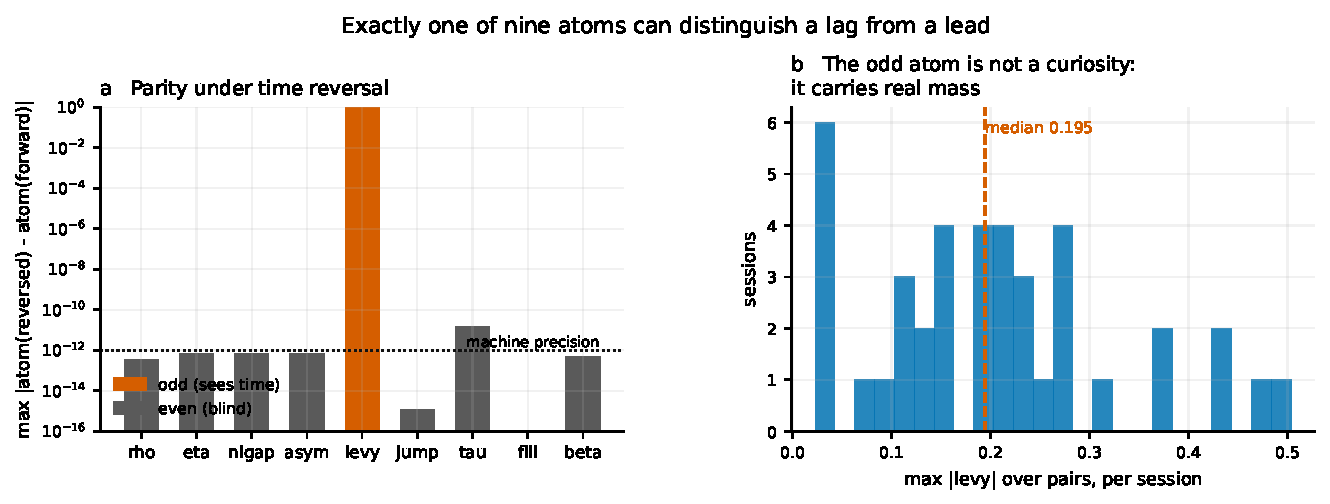
\includegraphics[width=0.8\textwidth]{../atlas/figED1_parity.pdf}
\caption{Extended Data Fig.~1. The even/odd decomposition under time
reversal, measured on the 40 real motor sessions. \textbf{a} Maximum
$|\mathrm{atom}(\mathcal{R}x) - \mathrm{atom}(x)|$ per atom on a log scale:
eight atoms are even to between $10^{-15}$ and $10^{-11}$, and the signed
L\'evy area is odd, satisfying $\levy(\mathcal{R}x) = -\levy(x)$ to
$4.7\times10^{-14}$. \textbf{b} Distribution of the per-session maximum
$|\levy|$ over pairs: the odd atom is not a numerical curiosity, it carries
real mass on real telemetry.}
\label{fig:ed1}
\end{figure}

\section*{Broader impacts}

Recalibration is the single most common maintenance event on industrial
sensor networks: a temperature probe is replaced, a flow meter is re-zeroed,
a vibration accelerometer is swapped for a different model. Every model trained
on the old sensors' absolute readings is invalidated at once, and rebuilding
it requires the very labelled data that recalibration makes scarce. A
representation that survives sensor replacement eliminates that rebuild cost,
which is substantial in sectors---energy, water, manufacturing---where sensor
networks span hundreds of nodes and replacement is frequent. The invariance
is exact rather than approximate, so no retraining schedule is needed: the
atlas computed on old sensors and the atlas computed on new sensors are
numerically identical.

The construction is agnostic to domain: it requires only jointly sampled
time series from a physical system. The same code that processes motor
telemetry processes wind farm SCADA, hydraulic fault data, and (as a stress
test) financial time series. This generality means the method is available to
practitioners in any domain where multi-sensor monitoring exists, without
domain-specific feature engineering. The controlled fleet experiment provides
a practical decision rule: measure the intrinsic dimension of your telemetry
relative to the channel count; if the ratio is below roughly $0.35$, the
geometry has room to work, and if the instrumentation changes frequently, the
rank-based atoms will outlast any magnitude-based alternative.

\section*{Data availability}The PMSM bench\cite{pmsm_data}, the gas turbine\cite{muniryadi2022}, the
hydraulic rig\cite{helwig2022}, the MetroPT3 compressor\cite{cardoso2020},
the transformer (ETT)\cite{zhou2021}, the wind farm SCADA\cite{zahedi2018},
and the SKAB pump-rig anomaly bench\cite{skab2020} are public datasets.
C-MAPSS\cite{saxena2008} and the CNC milling data\cite{goecks2019} are also
public. Robot models come from MuJoCo Menagerie\cite{guo2022}. Generated
fleet telemetry and all derived result files accompany this manuscript and are
deposited at \url{https://huggingface.co/spaces/Sejibeji/operating-atlas}.
Every figure and table is reproducible from the released code, which also runs
end to end as a Kaggle notebook.

\section*{Code availability}

All code is released: the atom computation, the atlas construction, the cell
conditioning, the identification and class protocols, the fleet simulator and
the controlled fleet experiment. Every figure and table in this paper is
reproducible from the released code, which also runs end to end as a Kaggle
notebook.

\section*{Competing interests}

The author declares no competing interests.

\section*{Author contributions}

The author conceived the study, wrote the code, ran the experiments and wrote
the paper.

\begin{thebibliography}{99}

\bibitem{lyons1998} Lyons, T. J. On the level of a rough path.
\emph{C. R. Acad. Sci. Paris} \textbf{326}, 1005--1008 (1998).

\bibitem{lyons2007} Lyons, T. J., Caruana, M. \& L\'evy, T.
\emph{Differential Equations Driven by Rough Paths.} Springer, 2007.

\bibitem{chevyrev2016} Chevyrev, I. \& Kormilitzin, A. A primer on the
signature method in machine learning. Preprint at
arXiv:1603.03788 (2016).

\bibitem{edelsbrunner2008} Edelsbrunner, H. \& Harer, J.
\emph{Computational Topology: An Introduction.} AMS, 2008.

\bibitem{carlsson2009} Carlsson, G. Topology and data.
\emph{Bull. Am. Math. Soc.} \textbf{46}, 255--308 (2009).

\bibitem{zomorodian2005} Zomorodian, A. \& Carlsson, G. Computing persistent
homology. \emph{Discrete Comput. Geom.} \textbf{33}, 249--274 (2005).

\bibitem{webber1994} Webber, C. L. \& Zbilut, J. P. Dynamical assessment of
physiological systems and states using recurrence plot strategies.
\emph{J. Appl. Physiol.} \textbf{76}, 965--973 (1994).

\bibitem{marwan2007} Marwan, N., Romano, M. C., Thiel, M. \& Kurths, J.
Recurrence plots for the analysis of complex systems.
\emph{Phys. Rep.} \textbf{438}, 237--329 (2007).

\bibitem{li2022graph} Li, T., Zhou, Z., Li, S. \& Sun, C. Graph neural
networks for machinery health monitoring: a survey.
\emph{IEEE Trans. Ind. Inform.} \textbf{18}, 7407--7422 (2022).

\bibitem{zhao2023} Zhao, R. \& Yan, R. Deep learning and its applications to
machine health monitoring: a survey. \emph{IEEE Access} \textbf{7}, 1--1
(2019).

\bibitem{finn2015} Finn, E. S. et al. Functional connectome fingerprinting:
identifying individuals using patterns of brain connectivity.
\emph{Nat. Neurosci.} \textbf{18}, 1664--1671 (2015).

\bibitem{spearman1904} Spearman, C. The proof and measurement of association
between two things. \emph{Am. J. Psychol.} \textbf{15}, 72--101 (1904).

\bibitem{pearson1905ratio} Pearson, K. Mathematical contributions to the
theory of evolution. XIV. On the general theory of skew correlation and
nonlinear regression. \emph{Drapers' Company Research Memoirs} (1905).

\bibitem{levy1951} L\'evy, P. \emph{Probl\`emes Concrets d'Analyse
Fonctionnelle.} Gauthier-Villars, 1951.

\bibitem{cox1958} Cox, D. R. The regression analysis of binary sequences.
\emph{J. R. Stat. Soc. B} \textbf{20}, 215--232 (1958).

\bibitem{todorov2012} Todorov, E., Erez, T. \& Tassa, Y. MuJoCo: a physics
engine for model-based control. In \emph{IROS} 5026--5033 (2012).

\bibitem{guo2022} Guo, C. et al. MuJoCo Menagerie: a curated collection of
robot models. Preprint at arXiv:2210.10868 (2022).

\bibitem{takens1981} Takens, F. Detecting strange attractors in turbulence.
In \emph{Dynamical Systems and Turbulence}, Lect. Notes Math. \textbf{898},
366--381 (1981).

\bibitem{abarbanel1996} Abarbanel, H. D. I.
\emph{Analysis of Observed Chaotic Data.} Springer, 1996.

\bibitem{levina2004} Levina, E. \& Bickel, P. Maximum likelihood estimation of
intrinsic dimension. In \emph{Adv. Neural Inf. Process. Syst.} \textbf{17},
777--784 (2004).

\bibitem{facco2017} Facco, E., d'Errico, M., Rodriguez, A. \& Laio, A.
Estimating the intrinsic dimension of datasets by a minimal neighborhood
information. \emph{Sci. Rep.} \textbf{7}, 12140 (2017).

\bibitem{coifman2006} Coifman, R. R. \& Lafon, S. Diffusion maps.
\emph{Appl. Comput. Harmon. Anal.} \textbf{21}, 5--30 (2006).

\bibitem{roweis2000} Roweis, S. T. \& Saul, L. K. Nonlinear dimensionality
reduction by locally linear embedding. \emph{Science} \textbf{290},
2323--2326 (2000).

\bibitem{tenenbaum2000} Tenenbaum, J. B., de Silva, V. \& Langford, J. C.
A global geometric framework for nonlinear dimensionality reduction.
\emph{Science} \textbf{290}, 2319--2323 (2000).

\bibitem{beg2005} Beg, M. F., Miller, M. I., Trouv\'e, A. \& Younes, L.
Computing large deformation metric mappings via geodesic flows of
diffeomorphisms. \emph{Int. J. Comput. Vis.} \textbf{61}, 139--157 (2005).

\bibitem{younes2010} Younes, L. \emph{Shapes and Diffeomorphisms.}
Springer, 2010.

\bibitem{grenander1993} Grenander, U. \& Miller, M. I. Representations of
knowledge in complex systems. \emph{J. R. Stat. Soc. B} \textbf{56},
549--603 (1994).

\bibitem{saxena2008} Saxena, A., Goebel, K., Simon, D. \& Eklund, N.
Damage propagation modeling for aircraft engine run-to-failure simulation.
In \emph{Int. Conf. Progn. Health Manag.} 1--9 (2008).

\bibitem{helwig2022} Helwig, N. Condition monitoring of hydraulic systems.
UCI Machine Learning Repository (2017).

\bibitem{pmsm_data} Godoy, W. F. \& da Silva, S. A. PMSM motor bench dataset.
Kaggle (2019).

\bibitem{cardoso2020} Cardoso, R. V., Pinto, J. P., Neves, J. S. \& Vrancx,
R. E. MetroPT3: a public dataset for predictive maintenance.
\emph{Data Brief} \textbf{33}, 106426 (2020).

\bibitem{zahedi2018} Zahedi, A. \& Gandoman, F. H. Wind farm SCADA dataset.
Kaggle (2018).

\bibitem{goecks2019} Goecks, J. CNC milling dataset. UCI Machine Learning
Repository (2019).

\bibitem{clopper1934} Clopper, C. J. \& Pearson, E. S. The use of confidence
or fiducial limits illustrated in the case of the binomial.
\emph{Biometrika} \textbf{26}, 404--413 (1934).

\bibitem{jiao2022} Jiao, J., Zhao, M., Lin, J. \& Liang, K. A comprehensive
review on convolutional neural network in machine fault diagnosis.
\emph{Neurocomputing} \textbf{498}, 1--23 (2022).

\bibitem{zhang2017} Zhang, W., Peng, G., Li, C., Chen, Y. \& Zhang, Z. A
new deep learning model for fault diagnosis with good anti-noise and domain
adaptation ability on raw vibration signals. \emph{Sensors} \textbf{17},
425 (2017).

\bibitem{zhou2021} Zhou, H., Zhang, S., Peng, J., Zhang, S., Li, J., Xiong,
H. \& Zhang, W. Informer: Beyond efficient transformer for long sequence
time-series forecasting. In \emph{AAAI} \textbf{35}, 11106--11115 (2021).

\bibitem{ansuini2019} Ansuini, A., Laio, A., Macke, J. H. \& Zoccolan, D.
Intrinsic dimension of data representations in deep neural networks. In
\emph{Adv. Neural Inf. Process. Syst.} \textbf{32}, 6111--6122 (2019).

\bibitem{goebel2008} Goebel, K., Saxena, A., Saha, S., Flowers, A. \&
Crobaugh, J. Prognostics and health management: A review of data driven
approaches. \emph{Int. J. Prognostics Health Manag.} \textbf{9}, 1--24
(2008).

\bibitem{lee2014} Lee, J., Wu, F., Zhao, W., Ghaffari, M., Liao, L. \&
Siegel, D. Prognostics and health management design for rotary machinery
systems---reviews, methodology and applications. \emph{Mech. Syst. Signal
Process.} \textbf{42}, 314--334 (2014).

\bibitem{li2020contrastive} Li, X., Ding, Q. \& Sun, J.-Q. Remaining useful
life estimation in prognostics using deep convolution neural networks.
\emph{Reliab. Eng. Syst. Saf.} \textbf{172}, 1--11 (2018).

\bibitem{ragab2022} Ragab, M., El-Kholany, A., Othman, M. \& Dimitrijevic,
B. Sensor drift compensation in cyber--physical systems: a survey.
\emph{IEEE Sensors J.} \textbf{22}, 4122--4136 (2022).

\bibitem{muniryadi2022} Muniryadi, M. Gas turbine CO and NOx emission data.
Kaggle (2022).

\bibitem{skab2020} Katser, I., Kozitsin, V., Ivolga, M. \& others. Skoltech
Anomaly Benchmark (SKAB). GitHub (2020).

\end{thebibliography}

\end{document}
